\begin{table}[H]
    {\renewcommand{\arraystretch}{1.3}%
    \setlength{\tabcolsep}{0.3em}%
    \begin{tabular}{bababab}
    \toprule
\rowcolor{white} \null &
\textbf{Synthetic$_{\mathbf{\mathcal{F}}}$} & \textbf{Synthetic$_{\mathbf{\mathcal{\beta}}}$} &
\textbf{Lehrpfad$_{\mathbf{\mathcal{F}}}$} & \textbf{Lehrpfad$_{\mathbf{\mathcal{\beta}}}$} &
\textbf{Office$_{\mathbf{\mathcal{F}}}$} & \textbf{Office$_{\mathbf{\mathcal{\beta}}}$}
\\
\midrule
\rowcolor{lightgray}
\textbf{Keypoint Count} &
    \num{49469} & \num{45811} &
    \num{165916} & \num{159291} &
    \num{13417} & \num{12370}
    \\
\textbf{Correspondences} &
    \num{18593} & \num{16139} &
    \num{11023} & \num{6542} &
    \num{2303} & \num{872}
    \\
\rowcolor{lightgray}
\textbf{True Positives} &
    \num{11724} & \num{10039} &
    \num{4018} & \num{1370} &
    \num{1547} & \num{431}
    \\
\textbf{False Positives} &
    \num{10993} & \num{10520} &
    \num{53693} & \num{59940} &
    \num{3418} & \num{4215}
    \\
    \bottomrule
    \end{tabular}
    }
    \caption{Performance indicators for the default configuration of the SIFT algorithm on the different datasets.}
\end{table}

\begin{figure}[H]
\begin{subfigure}[t]{0.45\linewidth}
    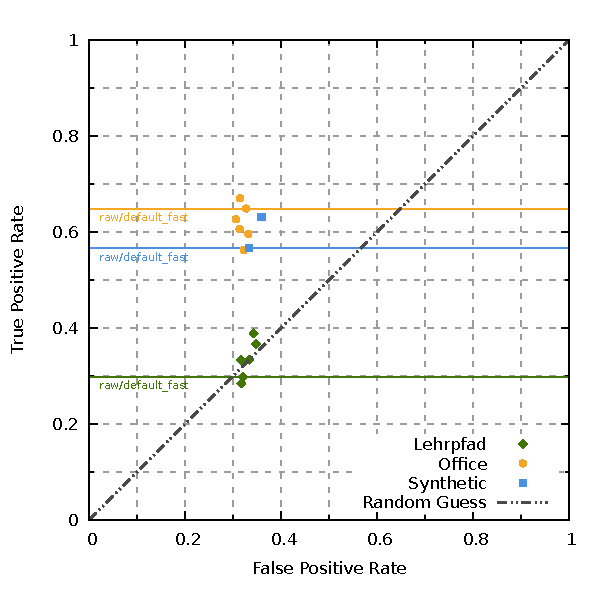
\includegraphics[width=\linewidth]{chapter06/results/ORB/flexion/roc.pdf}%
    \caption{Flexion Image ROC}
\end{subfigure}\quad
\begin{subfigure}[t]{0.45\linewidth}
    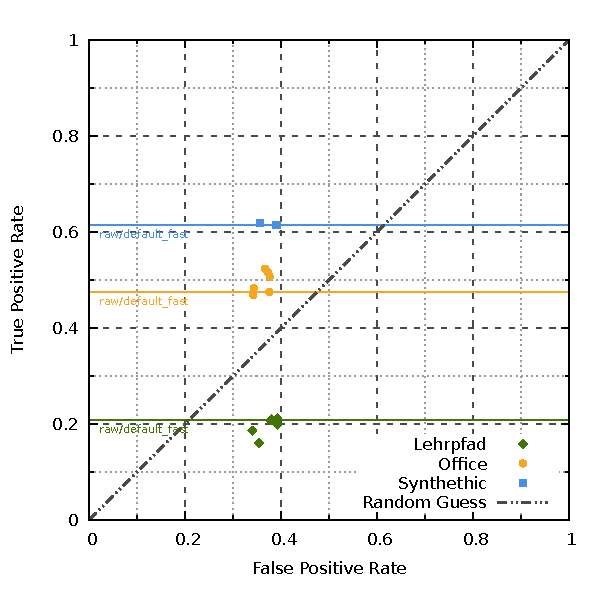
\includegraphics[width=\linewidth]{chapter06/results/ORB/bearing/roc.pdf}
    \caption{Bearing-Angle Image ROC}
\end{subfigure}
    \caption{ORB}
\end{figure}

\begin{figure}[H]
\begin{subfigure}[t]{0.45\linewidth}
    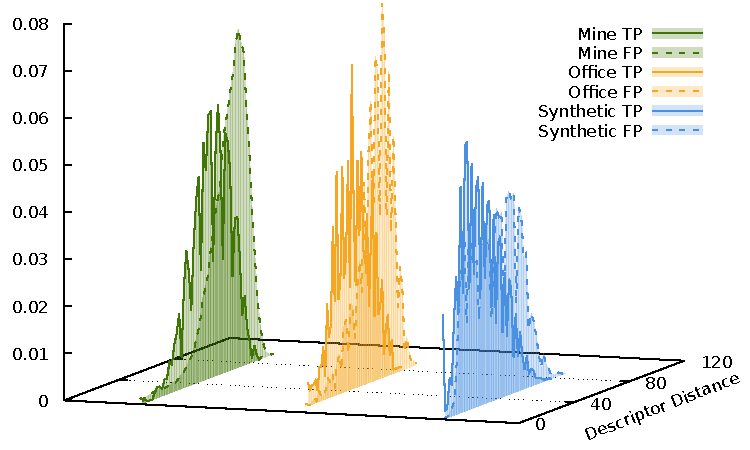
\includegraphics[width=\linewidth]{chapter06/results/ORB/flexion/descriptor_distances.pdf}%
    \caption{\gls{flexion-image} Descriptor Distances}
\end{subfigure}\quad
\begin{subfigure}[t]{0.45\linewidth}
    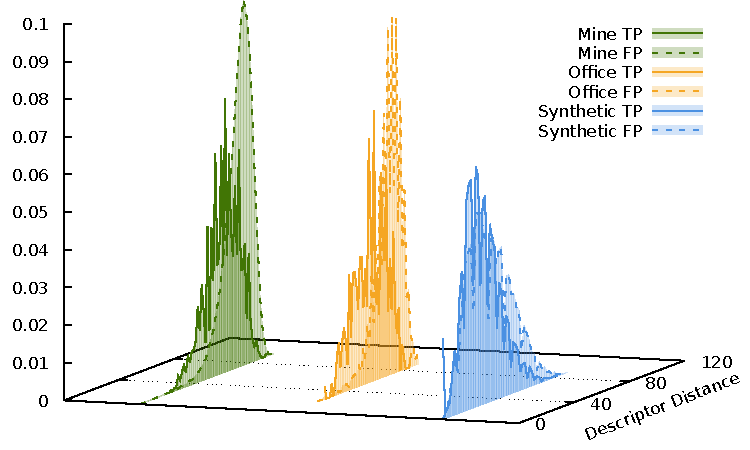
\includegraphics[width=\linewidth]{chapter06/results/ORB/bearing/descriptor_distances.pdf}%
    \caption{\gls{bearing-angle-image} Descriptors Distances}
\end{subfigure}
\end{figure}
